\begin{enumerate}[label=\thesection.\arabic*.,ref=\thesection.\theenumi]
\numberwithin{equation}{enumi}
\item
Consider the following second order system with the transfer function
\begin{align}
G(s) = \frac{1}{1+2s+s^2}
\end{align}
Is the system stable? 
\\
\solution 
\begin{align}
G(s) = \frac{1}{1+2s+s^2}
\end{align}
From given expression of G(s),both poles of G(s) are at (-1,0) which is on the left half of s-plane, therefore we can conclude that the system is stable.
\item Find and sketch the step response $c(t)$ of the system.
\\
\solution 
For step-response, we take input as unit-step function u(t)
\begin{align}
C(s) = R(s).G(s) = \sbrak{\frac{1}{s}} \sbrak{\frac{1}{1+2s+s^2}}
\end{align}

\begin{align}
C(s) =  \frac{1}{s(1+s)^2}
\end{align}



Using Partial Fractions,
\begin{align}
C(s) = \frac{1}{s} - \frac{1}{(1+s)} - \frac{1}{(1+s)^2}
\end{align}

%\end{frame}
%\begin{frame}{Inverse Laplace}
%$$c(t) = L^{-1} ( \frac{1}{s} - \frac{1}{(1+s)} - \frac{1}{(1+s)^2}) $$
%From the properties of inverse Laplace transform,
%$$L^{-1} (F_1(s) + F_2(s) + F_3(s)) = L^{-1}(F_1(s)) + L^{-1}(F_2(s)) + L^{-1}(F_3(s))$$

Therefore;
\begin{align}
c(t) = L^{-1} \sbrak{ \frac{1}{s}} - L^{-1}\sbrak{\frac{1}{1+s}} - L^{-1}\sbrak{\frac{1}{(1+s)^2}} 
\end{align}

Using the Known inverse transforms:
\begin{align}
c(t) = (1 - e^{-t} - te^{-t}) . u(t)
\end{align}
\lstinputlisting{./codes/ee18btech11002/plot.py}
\begin{figure}
\centering
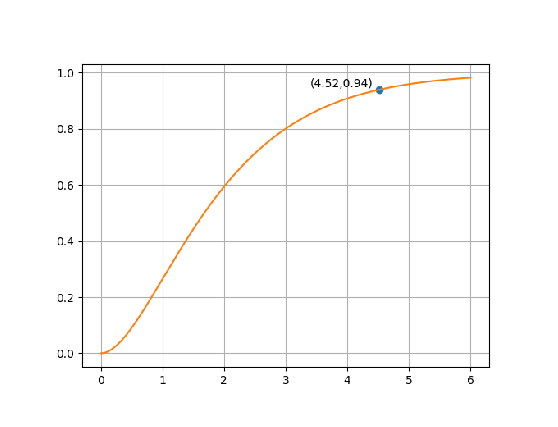
\includegraphics[width=\columnwidth]{./figs/ee18btech11002.eps}
\caption{}
\label{fig:sec_order}
\end{figure}
\item Find the steady state response of the system.
\\
\solution 
To know the steady response value of c(t), we calculate 
\begin{align}
\lim_{t\to\infty} c(t) = (1+0+0).(1) = 1
\end{align}

\item Find the time system output c(t) to reach 94\% of its steady state value.
\\
\solution 
Now, 94\% of 1 is 0.94, so we should now solve for a positive t such that
\begin{align}
(1 - e^{-t} - te^{-t}) = 0.94
\end{align}
\lstinputlisting{./codes/ee18btech11002/solution.py}
%the attached code gives us the solution for the equation
%and t turns out to be
\begin{align}
 t = 4.5228
\end{align}


 

%\end{frame}
%\begin{frame}{Finding the time for reaching 94\%}



%Therefore, answer is option (b)
%\end{frame}
%\begin{frame}{Plot}
%We can verify the solution by plotting c(t):

\end{enumerate}
